\documentclass{report}
% Include all project wide packages here.
\usepackage{fullpage}
\usepackage{polyglossia}
\setmainlanguage{dutch}
\usepackage{csquotes}
\usepackage{graphicx}
\usepackage{epstopdf}
\usepackage{pdfpages}
\usepackage{caption}
\usepackage[list=true]{subcaption}
\usepackage{float}
%\usepackage{mathtools}
\usepackage{standalone}
\usepackage{import}
\usepackage{tocloft}
\usepackage{wrapfig}
\usepackage{authblk}
\usepackage{array}
\usepackage{booktabs}
\usepackage[toc,page,title,titletoc]{appendix}
\usepackage{xunicode}
\usepackage{amsmath}
\usepackage{fontspec}
\usepackage{unicode-math}
\usepackage[
    backend=bibtexu,
	texencoding=utf8,
bibencoding=utf8,
    style=ieee,
    sortlocale=nl_NL,
    language=auto
]{biblatex}
\usepackage{listings}
\newcommand{\includecode}[3][c]{\lstinputlisting[caption=#2, escapechar=, style=#1]{#3}}
\newcommand{\superscript}[1]{\ensuremath{^{\textrm{#1}}}}
\newcommand{\subscript}[1]{\ensuremath{_{\textrm{#1}}}}


\newcommand{\chapternumber}{\thechapter}
\renewcommand{\appendixname}{Bijlage}
\renewcommand{\appendixtocname}{Bijlagen}
\renewcommand{\appendixpagename}{Bijlagen}

\usepackage[hidelinks]{hyperref} %<--------ALTIJD ALS LAATSTE

%\renewcommand{\familydefault}{\sfdefault}

\setmainfont[Ligatures=TeX]{Myriad Pro}
\setmathfont{Asana Math}
\setmonofont{Lucida Console}

\usepackage{titlesec, blindtext, color}
\definecolor{gray75}{gray}{0.75}
\newcommand{\hsp}{\hspace{20pt}}
\titleformat{\chapter}[hang]{\Huge\bfseries}{\chapternumber\hsp\textcolor{gray75}{|}\hsp}{0pt}{\Huge\bfseries}
\renewcommand{\familydefault}{\sfdefault}
\renewcommand{\arraystretch}{1.2}
\setlength\parindent{0pt}

%For code listings
\definecolor{black}{rgb}{0,0,0}
\definecolor{browntags}{rgb}{0.65,0.1,0.1}
\definecolor{bluestrings}{rgb}{0,0,1}
\definecolor{graycomments}{rgb}{0.4,0.4,0.4}
\definecolor{redkeywords}{rgb}{1,0,0}
\definecolor{bluekeywords}{rgb}{0.13,0.13,0.8}
\definecolor{greencomments}{rgb}{0,0.5,0}
\definecolor{redstrings}{rgb}{0.9,0,0}
\definecolor{purpleidentifiers}{rgb}{0.01,0,0.01}


\lstdefinestyle{csharp}{
language=[Sharp]C,
showspaces=false,
showtabs=false,
breaklines=true,
showstringspaces=false,
breakatwhitespace=true,
escapeinside={(*@}{@*)},
columns=fullflexible,
commentstyle=\color{greencomments},
keywordstyle=\color{bluekeywords}\bfseries,
stringstyle=\color{redstrings},
identifierstyle=\color{purpleidentifiers},
basicstyle=\ttfamily\small}

\lstdefinestyle{c}{
language=C,
showspaces=false,
showtabs=false,
breaklines=true,
showstringspaces=false,
breakatwhitespace=true,
escapeinside={(*@}{@*)},
columns=fullflexible,
commentstyle=\color{greencomments},
keywordstyle=\color{bluekeywords}\bfseries,
stringstyle=\color{bluestrings},
identifierstyle=\color{purpleidentifiers}
}

\lstdefinestyle{vhdl}{
language=VHDL,
showspaces=false,
showtabs=false,
breaklines=true,
showstringspaces=false,
breakatwhitespace=true,
escapeinside={(*@}{@*)},
columns=fullflexible,
commentstyle=\color{greencomments},
keywordstyle=\color{bluekeywords}\bfseries,
stringstyle=\color{redstrings},
identifierstyle=\color{purpleidentifiers}
}

\lstdefinestyle{xaml}{
language=XML,
showspaces=false,
showtabs=false,
breaklines=true,
showstringspaces=false,
breakatwhitespace=true,
escapeinside={(*@}{@*)},
columns=fullflexible,
commentstyle=\color{greencomments},
keywordstyle=\color{redkeywords},
stringstyle=\color{bluestrings},
tagstyle=\color{browntags},
morestring=[b]",
  morecomment=[s]{<?}{?>},
  morekeywords={xmlns,version,typex:AsyncRecords,x:Arguments,x:Boolean,x:Byte,x:Char,x:Class,x:ClassAttributes,x:ClassModifier,x:Code,x:ConnectionId,x:Decimal,x:Double,x:FactoryMethod,x:FieldModifier,x:Int16,x:Int32,x:Int64,x:Key,x:Members,x:Name,x:Object,x:Property,x:Shared,x:Single,x:String,x:Subclass,x:SynchronousMode,x:TimeSpan,x:TypeArguments,x:Uid,x:Uri,x:XData,Grid.Column,Grid.ColumnSpan,Click,ClipToBounds,Content,DropDownOpened,FontSize,Foreground,Header,Height,HorizontalAlignment,HorizontalContentAlignment,IsCancel,IsDefault,IsEnabled,IsSelected,Margin,MinHeight,MinWidth,Padding,SnapsToDevicePixels,Target,TextWrapping,Title,VerticalAlignment,VerticalContentAlignment,Width,WindowStartupLocation,Binding,Mode,OneWay,xmlns:x}
}

%defaults
\lstset{
basicstyle=\ttfamily\small,
extendedchars=false,
numbers=left,
numberstyle=\ttfamily\tiny,
stepnumber=1,
tabsize=4,
numbersep=5pt
}

\begin{document}
\newcommand{\rp}{$\rightarrow$}
\newcommand{\Ohm}{$\Omega$}
\newcommand{\ohm}{$\omega$}
\newcommand{\gmu}{$\mu$}
\newcommand{\tss}{\textsubscript}
\newcommand{\lijst}{\lstinputlisting}

%%%%%%%%%%%%%%%%%%%%%%%%%%%%%%%%%%%%%%%%%
% University Assignment Title Page 
% LaTeX Template
% Version 1.0 (27/12/12)
%
% This template has been downloaded from:
% http://www.LaTeXTemplates.com
%
% Original author:
% WikiBooks (http://en.wikibooks.org/wiki/LaTeX/Title_Creation)
%
% License:
% CC BY-NC-SA 3.0 (http://creativecommons.org/licenses/by-nc-sa/3.0/)
% 
% Instructions for using this template:
% This title page is capable of being compiled as is. This is not useful for 
% including it in another document. To do this, you have two options: 
%
% 1) Copy/paste everything between \begin{document} and \end{document} 
% starting at \begin{titlepage} and paste this into another LaTeX file where you 
% want your title page.
% OR
% 2) Remove everything outside the \begin{titlepage} and \end{titlepage} and 
% move this file to the same directory as the LaTeX file you wish to add it to. 
% Then add %%%%%%%%%%%%%%%%%%%%%%%%%%%%%%%%%%%%%%%%%
% University Assignment Title Page 
% LaTeX Template
% Version 1.0 (27/12/12)
%
% This template has been downloaded from:
% http://www.LaTeXTemplates.com
%
% Original author:
% WikiBooks (http://en.wikibooks.org/wiki/LaTeX/Title_Creation)
%
% License:
% CC BY-NC-SA 3.0 (http://creativecommons.org/licenses/by-nc-sa/3.0/)
% 
% Instructions for using this template:
% This title page is capable of being compiled as is. This is not useful for 
% including it in another document. To do this, you have two options: 
%
% 1) Copy/paste everything between \begin{document} and \end{document} 
% starting at \begin{titlepage} and paste this into another LaTeX file where you 
% want your title page.
% OR
% 2) Remove everything outside the \begin{titlepage} and \end{titlepage} and 
% move this file to the same directory as the LaTeX file you wish to add it to. 
% Then add %%%%%%%%%%%%%%%%%%%%%%%%%%%%%%%%%%%%%%%%%
% University Assignment Title Page 
% LaTeX Template
% Version 1.0 (27/12/12)
%
% This template has been downloaded from:
% http://www.LaTeXTemplates.com
%
% Original author:
% WikiBooks (http://en.wikibooks.org/wiki/LaTeX/Title_Creation)
%
% License:
% CC BY-NC-SA 3.0 (http://creativecommons.org/licenses/by-nc-sa/3.0/)
% 
% Instructions for using this template:
% This title page is capable of being compiled as is. This is not useful for 
% including it in another document. To do this, you have two options: 
%
% 1) Copy/paste everything between \begin{document} and \end{document} 
% starting at \begin{titlepage} and paste this into another LaTeX file where you 
% want your title page.
% OR
% 2) Remove everything outside the \begin{titlepage} and \end{titlepage} and 
% move this file to the same directory as the LaTeX file you wish to add it to. 
% Then add \input{./title_page_1.tex} to your LaTeX file where you want your
% title page.
%
%%%%%%%%%%%%%%%%%%%%%%%%%%%%%%%%%%%%%%%%%

%----------------------------------------------------------------------------------------
%	PACKAGES AND OTHER DOCUMENT CONFIGURATIONS
%----------------------------------------------------------------------------------------

\documentclass[12pt]{article}

\begin{document}

\begin{titlepage}

\newcommand{\HRule}{\rule{\linewidth}{0.5mm}} % Defines a new command for the horizontal lines, change thickness here

\center % Center everything on the page
 
%----------------------------------------------------------------------------------------
%	HEADING SECTIONS
%----------------------------------------------------------------------------------------

\textsc{\LARGE TU Delft}\\[1.5cm] % Name of your university/college
\textsc{\Large Moduleopdracht 4}\\[0.5cm] % Major heading such as course name
\textsc{\large EPO-3}\\[0.5cm] % Minor heading such as course title

%----------------------------------------------------------------------------------------
%	TITLE SECTION
%----------------------------------------------------------------------------------------

\HRule \\[0.4cm]
{ \huge \bfseries Capaciteiten}\\[0.4cm] % Title of your document
\HRule \\[1.5cm]
 
%----------------------------------------------------------------------------------------
%	AUTHOR SECTION
%----------------------------------------------------------------------------------------

\begin{minipage}{0.4\textwidth}
\begin{flushleft} \large
\emph{Author:}\\
Kees \textsc{Hogenhout} % Your name
Efraïm \textsc{Eland} %other name
\end{flushleft}
\end{minipage}
~
\begin{minipage}{0.4\textwidth}
\begin{flushright} \large
\emph{Supervisor:} \\
Dr. James \textsc{Smith} % Supervisor's Name
\end{flushright}
\end{minipage}\\[4cm]

% If you don't want a supervisor, uncomment the two lines below and remove the section above
%\Large \emph{Author:}\\
%John \textsc{Smith}\\[3cm] % Your name

%----------------------------------------------------------------------------------------
%	DATE SECTION
%----------------------------------------------------------------------------------------

{\large \today}\\[3cm] % Date, change the \today to a set date if you want to be precise

%----------------------------------------------------------------------------------------
%	LOGO SECTION
%----------------------------------------------------------------------------------------

%\includegraphics{Logo}\\[1cm] % Include a department/university logo - this will require the graphicx package
 
%----------------------------------------------------------------------------------------
% 

\textbf{Abstract} \\
Hierin wordt kort samengevat wat de inhoud van de opdracht is. De bedoeling is om de dikte van het gate-oxide te berekenen, gegeven de specificaties 
in de moduleopdracht. In dit verslag worden de keuzes besproken, die gemaakt moesten worden om tot het juist resultaat te komen. De manier van het 
bepalen gaat slechts via simulaties in Spice. Deze opdracht is dan ook in het kader van de opleiding Elektrical engineering en geen state-of-the-art transistor-rapport.  Uiteindelijk is de dikte van het gate-oxide van de nmos-transistor berekend aan de hand van de gate capaciteit van de NMOS-transistor. Hoe de gate capaciteit weer bepaald is, leest u in dit verslag. 

\vfill % Fill the rest of the page with whitespace

\end{titlepage}
\end{document} to your LaTeX file where you want your
% title page.
%
%%%%%%%%%%%%%%%%%%%%%%%%%%%%%%%%%%%%%%%%%

%----------------------------------------------------------------------------------------
%	PACKAGES AND OTHER DOCUMENT CONFIGURATIONS
%----------------------------------------------------------------------------------------

\documentclass[12pt]{article}

\begin{document}

\begin{titlepage}

\newcommand{\HRule}{\rule{\linewidth}{0.5mm}} % Defines a new command for the horizontal lines, change thickness here

\center % Center everything on the page
 
%----------------------------------------------------------------------------------------
%	HEADING SECTIONS
%----------------------------------------------------------------------------------------

\textsc{\LARGE TU Delft}\\[1.5cm] % Name of your university/college
\textsc{\Large Moduleopdracht 4}\\[0.5cm] % Major heading such as course name
\textsc{\large EPO-3}\\[0.5cm] % Minor heading such as course title

%----------------------------------------------------------------------------------------
%	TITLE SECTION
%----------------------------------------------------------------------------------------

\HRule \\[0.4cm]
{ \huge \bfseries Capaciteiten}\\[0.4cm] % Title of your document
\HRule \\[1.5cm]
 
%----------------------------------------------------------------------------------------
%	AUTHOR SECTION
%----------------------------------------------------------------------------------------

\begin{minipage}{0.4\textwidth}
\begin{flushleft} \large
\emph{Author:}\\
Kees \textsc{Hogenhout} % Your name
Efraïm \textsc{Eland} %other name
\end{flushleft}
\end{minipage}
~
\begin{minipage}{0.4\textwidth}
\begin{flushright} \large
\emph{Supervisor:} \\
Dr. James \textsc{Smith} % Supervisor's Name
\end{flushright}
\end{minipage}\\[4cm]

% If you don't want a supervisor, uncomment the two lines below and remove the section above
%\Large \emph{Author:}\\
%John \textsc{Smith}\\[3cm] % Your name

%----------------------------------------------------------------------------------------
%	DATE SECTION
%----------------------------------------------------------------------------------------

{\large \today}\\[3cm] % Date, change the \today to a set date if you want to be precise

%----------------------------------------------------------------------------------------
%	LOGO SECTION
%----------------------------------------------------------------------------------------

%\includegraphics{Logo}\\[1cm] % Include a department/university logo - this will require the graphicx package
 
%----------------------------------------------------------------------------------------
% 

\textbf{Abstract} \\
Hierin wordt kort samengevat wat de inhoud van de opdracht is. De bedoeling is om de dikte van het gate-oxide te berekenen, gegeven de specificaties 
in de moduleopdracht. In dit verslag worden de keuzes besproken, die gemaakt moesten worden om tot het juist resultaat te komen. De manier van het 
bepalen gaat slechts via simulaties in Spice. Deze opdracht is dan ook in het kader van de opleiding Elektrical engineering en geen state-of-the-art transistor-rapport.  Uiteindelijk is de dikte van het gate-oxide van de nmos-transistor berekend aan de hand van de gate capaciteit van de NMOS-transistor. Hoe de gate capaciteit weer bepaald is, leest u in dit verslag. 

\vfill % Fill the rest of the page with whitespace

\end{titlepage}
\end{document} to your LaTeX file where you want your
% title page.
%
%%%%%%%%%%%%%%%%%%%%%%%%%%%%%%%%%%%%%%%%%

%----------------------------------------------------------------------------------------
%	PACKAGES AND OTHER DOCUMENT CONFIGURATIONS
%----------------------------------------------------------------------------------------

\documentclass[12pt]{article}

\begin{document}

\begin{titlepage}

\newcommand{\HRule}{\rule{\linewidth}{0.5mm}} % Defines a new command for the horizontal lines, change thickness here

\center % Center everything on the page
 
%----------------------------------------------------------------------------------------
%	HEADING SECTIONS
%----------------------------------------------------------------------------------------

\textsc{\LARGE TU Delft}\\[1.5cm] % Name of your university/college
\textsc{\Large Moduleopdracht 4}\\[0.5cm] % Major heading such as course name
\textsc{\large EPO-3}\\[0.5cm] % Minor heading such as course title

%----------------------------------------------------------------------------------------
%	TITLE SECTION
%----------------------------------------------------------------------------------------

\HRule \\[0.4cm]
{ \huge \bfseries Capaciteiten}\\[0.4cm] % Title of your document
\HRule \\[1.5cm]
 
%----------------------------------------------------------------------------------------
%	AUTHOR SECTION
%----------------------------------------------------------------------------------------

\begin{minipage}{0.4\textwidth}
\begin{flushleft} \large
\emph{Author:}\\
Kees \textsc{Hogenhout} % Your name
Efraïm \textsc{Eland} %other name
\end{flushleft}
\end{minipage}
~
\begin{minipage}{0.4\textwidth}
\begin{flushright} \large
\emph{Supervisor:} \\
Dr. James \textsc{Smith} % Supervisor's Name
\end{flushright}
\end{minipage}\\[4cm]

% If you don't want a supervisor, uncomment the two lines below and remove the section above
%\Large \emph{Author:}\\
%John \textsc{Smith}\\[3cm] % Your name

%----------------------------------------------------------------------------------------
%	DATE SECTION
%----------------------------------------------------------------------------------------

{\large \today}\\[3cm] % Date, change the \today to a set date if you want to be precise

%----------------------------------------------------------------------------------------
%	LOGO SECTION
%----------------------------------------------------------------------------------------

%\includegraphics{Logo}\\[1cm] % Include a department/university logo - this will require the graphicx package
 
%----------------------------------------------------------------------------------------
% 

\textbf{Abstract} \\
Hierin wordt kort samengevat wat de inhoud van de opdracht is. De bedoeling is om de dikte van het gate-oxide te berekenen, gegeven de specificaties 
in de moduleopdracht. In dit verslag worden de keuzes besproken, die gemaakt moesten worden om tot het juist resultaat te komen. De manier van het 
bepalen gaat slechts via simulaties in Spice. Deze opdracht is dan ook in het kader van de opleiding Elektrical engineering en geen state-of-the-art transistor-rapport.  Uiteindelijk is de dikte van het gate-oxide van de nmos-transistor berekend aan de hand van de gate capaciteit van de NMOS-transistor. Hoe de gate capaciteit weer bepaald is, leest u in dit verslag. 

\vfill % Fill the rest of the page with whitespace

\end{titlepage}
\end{document}

\chapter{Inleiding}
In de inleiding beschrijf je het probleem wat je op wilt lossen, zonder al te diep hierop in te gaan. Je
geeft hier ook de motivatie en context van je werk (waar is het belangrijk voor, welk groter probleem
wordt hiermee opgelost of geadresseerd).

\documentclass{scrartcl} % scrartcl of scrreprt
% Include all project wide packages here.
\usepackage{fullpage}
\usepackage{polyglossia}
\setmainlanguage{dutch}
\usepackage{csquotes}
\usepackage{graphicx}
\usepackage{epstopdf}
\usepackage{pdfpages}
\usepackage{caption}
\usepackage[list=true]{subcaption}
\usepackage{float}
%\usepackage{mathtools}
\usepackage{standalone}
\usepackage{import}
\usepackage{tocloft}
\usepackage{wrapfig}
\usepackage{authblk}
\usepackage{array}
\usepackage{booktabs}
\usepackage[toc,page,title,titletoc]{appendix}
\usepackage{xunicode}
\usepackage{amsmath}
\usepackage{fontspec}
\usepackage{unicode-math}
\usepackage[
    backend=bibtexu,
	texencoding=utf8,
bibencoding=utf8,
    style=ieee,
    sortlocale=nl_NL,
    language=auto
]{biblatex}
\usepackage{listings}
\newcommand{\includecode}[3][c]{\lstinputlisting[caption=#2, escapechar=, style=#1]{#3}}
\newcommand{\superscript}[1]{\ensuremath{^{\textrm{#1}}}}
\newcommand{\subscript}[1]{\ensuremath{_{\textrm{#1}}}}


\newcommand{\chapternumber}{\thechapter}
\renewcommand{\appendixname}{Bijlage}
\renewcommand{\appendixtocname}{Bijlagen}
\renewcommand{\appendixpagename}{Bijlagen}

\usepackage[hidelinks]{hyperref} %<--------ALTIJD ALS LAATSTE

\renewcommand{\familydefault}{\sfdefault}

\setmainfont[Ligatures=TeX]{Myriad Pro}
\setmathfont{Asana Math}
\setmonofont{Lucida Console}

\usepackage{titlesec, blindtext, color}
\definecolor{gray75}{gray}{0.75}
\newcommand{\hsp}{\hspace{20pt}}
\titleformat{\chapter}[hang]{\Huge\bfseries}{\chapternumber\hsp\textcolor{gray75}{|}\hsp}{0pt}{\Huge\bfseries}
\renewcommand{\familydefault}{\sfdefault}
\renewcommand{\arraystretch}{1.2}
\setlength\parindent{0pt}

%For code listings
\definecolor{black}{rgb}{0,0,0}
\definecolor{browntags}{rgb}{0.65,0.1,0.1}
\definecolor{bluestrings}{rgb}{0,0,1}
\definecolor{graycomments}{rgb}{0.4,0.4,0.4}
\definecolor{redkeywords}{rgb}{1,0,0}
\definecolor{bluekeywords}{rgb}{0.13,0.13,0.8}
\definecolor{greencomments}{rgb}{0,0.5,0}
\definecolor{redstrings}{rgb}{0.9,0,0}
\definecolor{purpleidentifiers}{rgb}{0.01,0,0.01}


\lstdefinestyle{csharp}{
language=[Sharp]C,
showspaces=false,
showtabs=false,
breaklines=true,
showstringspaces=false,
breakatwhitespace=true,
escapeinside={(*@}{@*)},
columns=fullflexible,
commentstyle=\color{greencomments},
keywordstyle=\color{bluekeywords}\bfseries,
stringstyle=\color{redstrings},
identifierstyle=\color{purpleidentifiers},
basicstyle=\ttfamily\small}

\lstdefinestyle{c}{
language=C,
showspaces=false,
showtabs=false,
breaklines=true,
showstringspaces=false,
breakatwhitespace=true,
escapeinside={(*@}{@*)},
columns=fullflexible,
commentstyle=\color{greencomments},
keywordstyle=\color{bluekeywords}\bfseries,
stringstyle=\color{bluestrings},
identifierstyle=\color{purpleidentifiers}
}

\lstdefinestyle{vhdl}{
language=VHDL,
showspaces=false,
showtabs=false,
breaklines=true,
showstringspaces=false,
breakatwhitespace=true,
escapeinside={(*@}{@*)},
columns=fullflexible,
commentstyle=\color{greencomments},
keywordstyle=\color{bluekeywords}\bfseries,
stringstyle=\color{redstrings},
identifierstyle=\color{purpleidentifiers}
}

\lstdefinestyle{xaml}{
language=XML,
showspaces=false,
showtabs=false,
breaklines=true,
showstringspaces=false,
breakatwhitespace=true,
escapeinside={(*@}{@*)},
columns=fullflexible,
commentstyle=\color{greencomments},
keywordstyle=\color{redkeywords},
stringstyle=\color{bluestrings},
tagstyle=\color{browntags},
morestring=[b]",
  morecomment=[s]{<?}{?>},
  morekeywords={xmlns,version,typex:AsyncRecords,x:Arguments,x:Boolean,x:Byte,x:Char,x:Class,x:ClassAttributes,x:ClassModifier,x:Code,x:ConnectionId,x:Decimal,x:Double,x:FactoryMethod,x:FieldModifier,x:Int16,x:Int32,x:Int64,x:Key,x:Members,x:Name,x:Object,x:Property,x:Shared,x:Single,x:String,x:Subclass,x:SynchronousMode,x:TimeSpan,x:TypeArguments,x:Uid,x:Uri,x:XData,Grid.Column,Grid.ColumnSpan,Click,ClipToBounds,Content,DropDownOpened,FontSize,Foreground,Header,Height,HorizontalAlignment,HorizontalContentAlignment,IsCancel,IsDefault,IsEnabled,IsSelected,Margin,MinHeight,MinWidth,Padding,SnapsToDevicePixels,Target,TextWrapping,Title,VerticalAlignment,VerticalContentAlignment,Width,WindowStartupLocation,Binding,Mode,OneWay,xmlns:x}
}

%defaults
\lstset{
basicstyle=\ttfamily\small,
extendedchars=false,
numbers=left,
numberstyle=\ttfamily\tiny,
stepnumber=1,
tabsize=4,
numbersep=5pt
}
\addbibresource{../../library/bibliography.bib}

\author{}
\title{EPO3: Eindrapport - Inleiding}

\begin{document}
\chapter{Inleiding}
\label{ch:inleiding}

In het kader van onze studie waar EPO-3 deel van uitmaakt hebben we een chip ontworpen. Deze chip is ontworpen omdat dit we EPO-3 project succesvol af willen ronden, en zo de punten kunnen behalen voor onze studie.\\
Dit verslag beschrijft de verschillende onderdelen die tot het ontwerp behoren en het daarbij behorende procesverloop. Eerst zullen de ontwerpspecificaties worden behandeld. Daarna wordt er per blok in ons ontwerp besproken wat de specificaties zijn, hoe de VHDL code werkt, het testplan, de synthese, switchleven en de extracted worden behandeld. Het algemene testplan en resultaten van ons totaalontwerp worden daarna behandeld waarbij alle blokken samenkomen. Tot slot wordt er nog gekeken naar het procesverloop en een conclusie en discussie uit het algehele project getrokken.


\end{document}

\chapter{Probleemstelling}
De probleemstelling kan bij een beknopt rapport als deze wellicht volledig in de inleiding verwerkt
worden. In sommige gevallen is het beter om een letterlijke kopie van de opdracht op te nemen, in
andere gevallen is het beter om de opdracht in eigen woorden op te nemen met daaromheen je eigen
interpretatie. Wanneer de opdracht niet voldoende eenduidig gespecificeerd is, bijvoorbeeld, moet je
aangeven hoe je die verder ingeperkt hebt.



Bepaal door middel van simulaties aan een transitor de dikte van het gate oxide. Daarvoor moet je eerst de gate-channel capaciteit per oppervlakte-eenheid bepalen. Hou er rekening mee dat de totale capaciteit ook nog een bijdrage kent van de zogenaamde \emph{lateral diffusion}. De totale capaciteit \emph{C\tss{G}} wordt dan beschreven door de volgende formule, met \emph{W} de breedte, \emph{L} de lengte van de transistor, \emph{C\tss{o}} de zogenaamde overlap capaciteit en \emph{C\tss{GC}} de gezochte kanaalcapaciteit:
\begin{equation}
\emph{C\tss{G} = W \ast C\tss{o} + L \ast W \ast C\tss{GC}}
\end{equation}
Door transistoren met verschillende afmetingen te nemen kun je de termen \emph{C\tss{o}} en \emph{C\tss{GC}} apart bepalen. Wanneer je \emph{C\tss{GC}} hebt, kun je met behulp van de permittiviteit van het gate materiaal (silicium dioxide, \emph{SiO\tss{2}}) de gezochte oxide dikte bepalen. In voorbeeld 3.9 van het boek van Rabaey [1] wordt uitgelegd hoe je de totale gate capaciteit kunt bepalen door middel van simulatie. Hou er rekening mee dat je alleen op zoek bent naar het vlakke deel van de grafiek in figuur 3.32 van Rabaey [1]. Dit vlakke deel is gelijk aan de waarde \emph{WLC\tss{ox}} in figuur 3.31 van Rabaey [1]. Doe de simulaties en berekeningen voor zowel de NMOS transistor als de PMOS transistor en bespreek de resultaten.





\chapter{Aanpak}
De kern van het rapport kan uiteen vallen in verschillende delen, bijvoorbeeld een eerste gedeelte
met achtergrondkennis en -theorie, en een volgend gedeelte met je eigen werk. Het eerste stuk
heeft dan tot doel om de theorie zodanig samen te vatten dat de rest van het rapport gemakkelijker
begrepen kan worden. Het hoofdgedeelte kan uit meerdere secties bestaan, het hangt heel sterk van
het onderwerp af wat dan de beste indeling is. Een min of meer gebruikelijke indeling is achtergrond
kennis - methode (opzet van experimenten) - resultaten, maar dat is niet meer dan een vuistregel.



\section{Theorie}


De gate van de MOS transistor is ge\"isoleerd van het geleidende kanaal door middel van het gate oxide, die een capaciteit heeft van:
\begin{equation}
C\tss{ox} = \frac{\epsilon\tss{ox}}{t\tss{ox}}
\end{equation} 
waarbij \emph{$\epsilon$\tss{ox}} de permittiviteit is van het oxide en \emph{t\tss{ox}} de dikte is van het oxide.
\\
De totale waarde van deze capaciteit heet de gate capaciteit \emph{C\tss{G}} en hangt onder andere af van de overlap capaciteit per lengte-eenheid \emph{C\tss{o}} en de gate-channel capaciteit per oppervlakte-eenheid \emph{C\tss{GC}}. Ook spelen de breedte \emph{W} en de lengte \emph{L} een rol. De volgende formule geeft het verband weer tussen deze variabelen:
\begin{equation}
C\tss{G} = W \ast C\tss{o} + L \ast W \ast C\tss{GC}
\end{equation}
De overlap capaciteit is de capaciteit die ontstaat doordat de grenzen van de source en de drain een klein stukje onder de gate zitten. Aangezien de gate en de source en drain van lading verschillen ontstaat hier een capaciteit die afhangt van de breedte \emph{W}. De \emph{G\tss{GC}} hangt af van de \emph{$\epsilon$\tss{ox}} en de t\tss{ox}, dus:
\begin{equation}
C\tss{GC} = C\tss{ox} = \frac{\epsilon\tss{ox}}{t\tss{ox}}
\end{equation}
Stel nu dat wij een schakeling maken zoals in figuur \ref{res:RABAEY_SCHAKELING} en het resultaat plotten in een grafiek met op de y-as de gate capaciteit \emph{C\tss{GC}} en op de x-as gate source spanning \emph{V\tss{GS}}. Dan ziet de grafiek eruit als in figuur \ref{res:RABAEY_CAP_PLOT}.

 \begin{figure} [h!]
 \begin{center}
 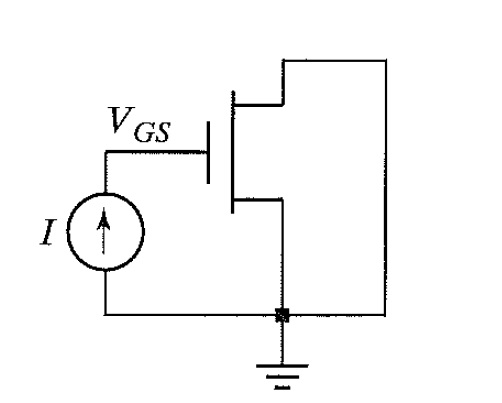
\includegraphics [scale = 0.7] {figures/RABAEY_SCHAKELING}
 \caption{Circuit om de gate capaciteit te bepalen van een NMOS transistor in 25$\mu$m technologie uit Rabaey [1]}
 \label{res:RABAEY_SCHAKELING}
 \end{center}
 \end{figure}

 \begin{figure} [h!]
 \begin{center}
 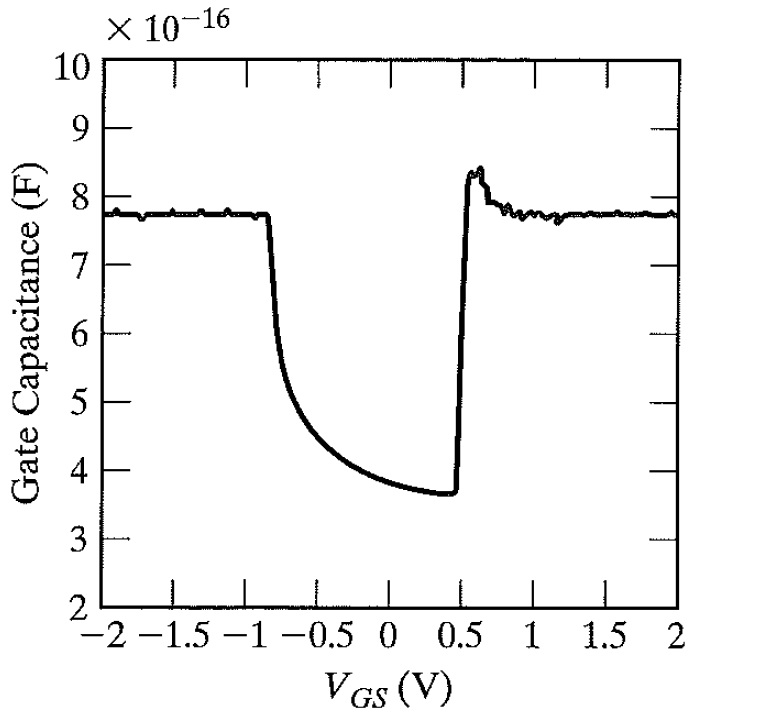
\includegraphics [scale = 0.4] {figures/RABAEY_CAP_PLOT}
 \caption{Plot van de \emph{C\tss{GC}}  \emph{V\tss{GS}} van een NMOS transistor in 25$\mu$m technologie uit Rabaey [1]}
 \label{res:RABAEY_CAP_PLOT}
 \end{center}
 \end{figure}

Uit figuur \ref{res:RABAEY_CAP_PLOT} is duidelijk te zien dat de \emph{C\tss{GC}} niet constant is voor elke \emph{V\tss{GS}}. Dit komt door de verschillende werkgebieden van de transistor. In figuur \ref{res:RABAEY_REGIONS} is een schematische weergave gegeven van drie verschillende werkgebieden. De verandering in capaciteitswaarde van de \emph{C\tss{GC}} is als volgt te verklaren: in het eerste vlakke gedeelte van figuur \ref{res:RABAEY_CAP_PLOT} zit de weerstand in het cut-off werkgebied. Er loopt geen stroom tussen source en drain. Naarmate de \emph{V\tss{GS}} stijgt, wordt de \emph{C\tss{GC}} kleiner. Dit komt omdat het p-substraat dat onder het gate oxide zit steeds verder naar beneden wordt gedrukt. Hierdoor wordt de afstand groter en dus de \emph{C\tss{GC}} kleiner. Zodra de \emph{V\tss{GS}} verder stijgt komt de transistor in het resistieve gebied. In dit gebied gaat een stroom tussen source en drain lopen. Hierdoor bereikt de \emph{C\tss{GC}} een constante waarde. Uit deze constante waarde kan men de dikte van het oxide afleiden. Het saturatie werkgebied van de transistor is voor dit verslag niet van belang en zal daarom hier niet worden besproken.

 \begin{figure} [h!]
 \begin{center}
 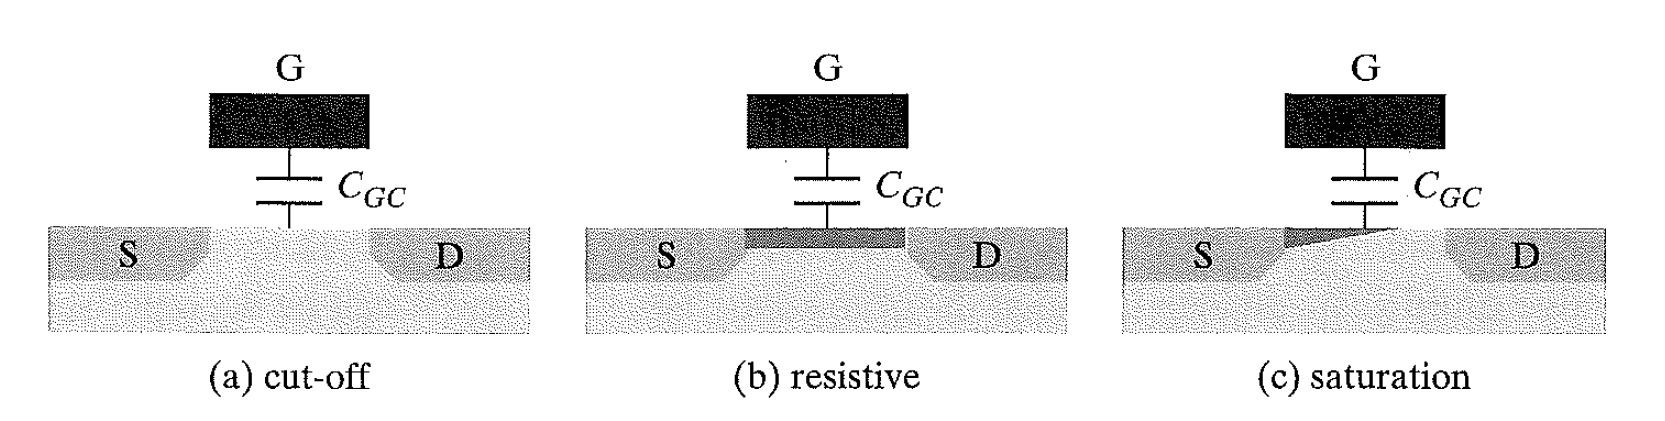
\includegraphics [scale = 0.4] {figures/RABAEY_REGIONS}
 \caption{Drie verschillende werkgebieden van een NMOS transistor uit Rabaey [1]}
 \label{res:RABAEY_REGIONS}
 \end{center}
 \end{figure}































\section{Eisen}



\section{Methode}


De methode valt uiteen in twee delen: Het bepalen van de t-90\% van een inverter en het bepalen van de t-90\% van drie inverters in cascade. 
\begin{enumerate}
\item Voor de eerste simulatie is het circuit in \ref{E1} gebruikt. De opdracht was om een enkele inverter te tekenen met een C\tss{load} van 25pF. Vervolgens diende deze gesimuleerd te worden bij een veranderende V6. Hierop moet dan een scope gezet worden om het ingangssignaal direct te zien. Bij "simulation parameters" dient dan een transient analyse aangevinkt te worden, om tegen de tijd te simuleren. De resultaten hiervan staan onder het kopje resultaten. 

\begin{figure} [h!]
\centering
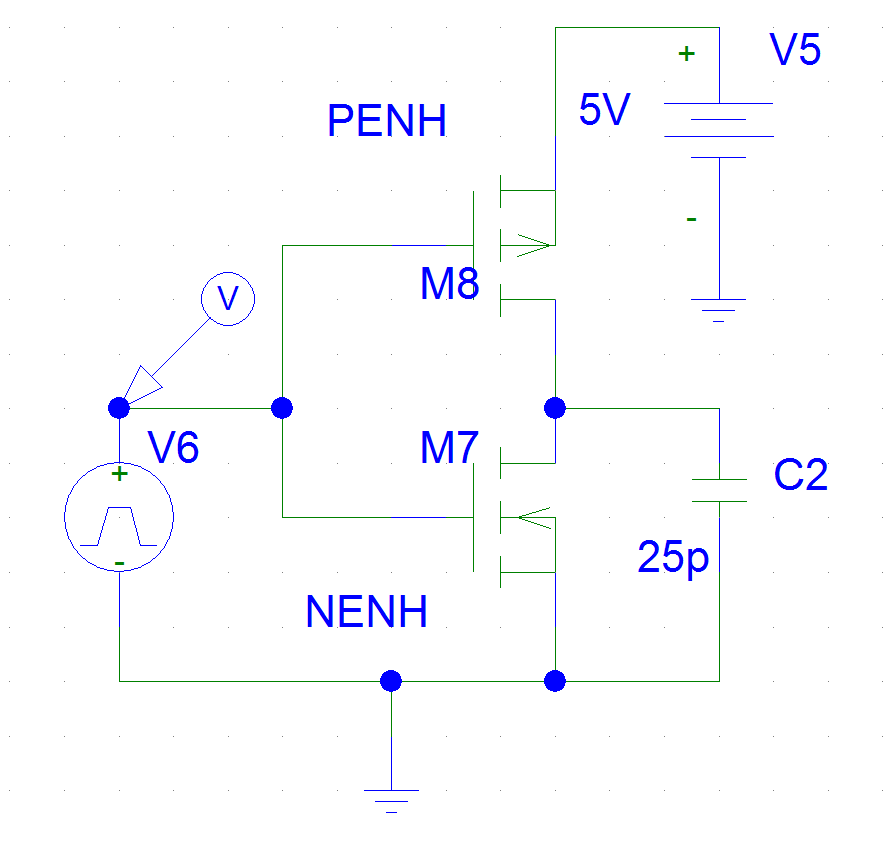
\includegraphics [scale = 0.4] {inputfiles/Inverter_circuit}
\caption{Het circuit van de enkele inverter in SPICE}
\label{E1}
\end{figure}
\newpage
\item Voor de tweede simulatie werd gevraagd om 3 inverters te simuleren. De eerste inverter is een normale inverter volgens de library die bij de opdracht gegeven is. De tweede inverter heeft een 5 keer zo grote breedte dan de eerste inverter en de derde inverter heeft een $5^2$ keer zo grote breedte als de eerste transistor. De bedoeling is dan om te onderzoeken of deze schakeling een bufferende werking heeft. De schakeling die hiervoor ontworpen is, staat in figuur \ref{E2}. De resultaten van de simulatie worden,  zoals eerder gezegd, hieronder besproken. 
\begin{figure} [h!]
\centering
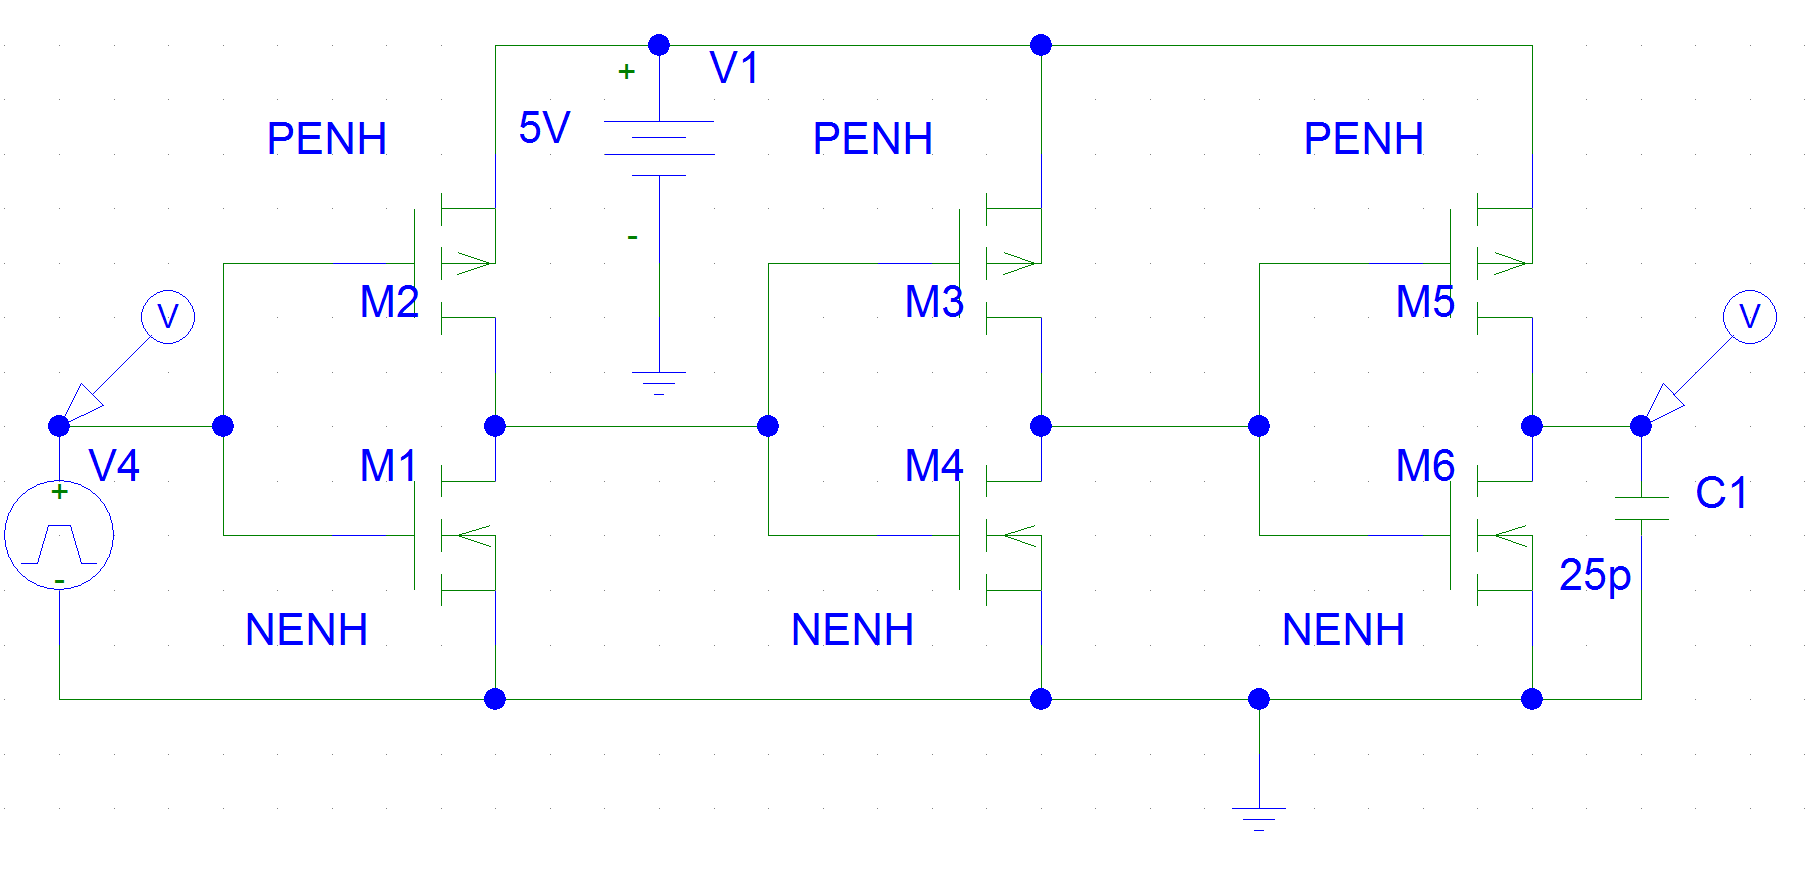
\includegraphics [width = \textwidth] {inputfiles/Cascade_circuit}
\caption{Het circuit van de driedubbele inverter in SPICE}
\label{E2}
\end{figure}
\end{enumerate}



\chapter{Resultaten}

\section{Plain results}



\begin{table} [h!]
\centering % 
\begin{tabular}{l c c c c c} 
\toprule % Top horizontal line
& \multicolumn {4}{c}{Formula variables} \\ % Amalgamating several columns into one cell is done using the \multicolumn command as seen on this line
\cmidrule(l){1-3} % Horizontal line spanning less than the full width of the table - you can add (r) or (l) just before the opening curly bracket to shorten the rule on the left or right side
L($\mu$m)&  W($\mu$m)  & C\tss{g}\\ % Column names row
\midrule % In-table horizontal line
2.2 & 3.0  & 8.3381 \\ % Content row 1
2.4 & 3.0 & 9.1672 \\ % Content row 2
2.8 & 3.0 & 10.825 \\ % Content row 3
3.2 & 3.0 & 12.483 \\ % Content row 4
3.6 & 3.0 & 14.141 \\ % Content row 5
4.0 & 3.0 & 15.799 \\ % Content row 6
4.4 & 3.0 & 17.457 \\ % Content row 7
4.8 & 3.0 & 19.115 \\ % Content row 8
\midrule % In-table horizontal line
\midrule % In-table horizontal line
%Average Rate & 0.920 & 0.882 \\ % Summary/total row
\bottomrule % Bottom horizontal line
\end{tabular}
\caption{Table caption text} % Table caption, can be commented out if no caption is required
\label{tab:template} % A label for referencing this table elsewhere, references are used in text as \ref{label}
\end{table}




\section{Analyse}
\chapter {Discussie}
In de ‘discussie’ sectie reflecteer je op de resultaten. Een uitkomst zonder discussie en/of reflectie
heeft zelden ‘impact’. Welke doelen zijn wel bereikt, welke niet. Komt je resultaat overeen met de
verwachte uitkomst? Zo niet, wat zou de oorzaak van het verschil kunnen zijn? Wat zijn de sterkepunten van je werk, en welke de zwakke? Wat zou je een andere keer anders doen? Bespreek, indien
van toepassing, implicaties, van je werk. Voorbeeld: wat is het mogelijke gevolg van Neutrino’s die
sneller reizen dan het licht? Wat zijn mogelijke bronnen van meetfouten of interpretatiefouten?

\chapter{Conclusie}
De conclusie is zeer belangrijk. Deze is meestal relatief kort, en vat heel beknopt de resultaten en
belangrijkste reflectie daarop nog eens samen. Wanneer de conclusie te lang zou worden, is het beter
om een aparte discussie sectie (zie hierboven) toe te voegen. In de conclusie kun je, indien van
toepassing, aanbevelingen doen voor verder werk/onderzoek. (Indien dat te lang zou worden, kun je
daar ook weer een aparte sectie van maken.) In de conclusie maak je ook eventuele slotopmerkingen.
Hou er rekening mee dat er lezers zijn die alleen het abstract en de conclusie lezen, en maak deze
stukken ook voor hen nuttig, bijvoorbeeld om te beslissen of ze het gehele rapport gaan lezen

\section{Conclusie}
\section{Discussie}



\chapter{Appendix}
\section{Matlab code}
\subsection{Matlab code om Cg vs. L te plotten}
\label{M1}
\lijst{inputfiles/c0.m}

\subsection{Bereken de dikte van het gate-oxide}
\label{M2}
\lijst{inputfiles/gateoxide.m}

\end{document}